\documentclass[12pt,a4paper]{article}
\usepackage[utf8]{inputenc}
\usepackage[T1]{fontenc}
\usepackage{amsmath}
\usepackage{amsfonts}
\usepackage{amssymb}
\usepackage{graphicx}
\usepackage[left=2.54cm, right=2.54cm, top=2.54cm, bottom=2.54cm]{geometry}
\usepackage[hidelinks]{hyperref} %for reference automatically
\usepackage{fancyhdr}
\usepackage{subcaption}

\usepackage{tikz}
\usetikzlibrary{positioning}

\pagestyle{fancy} % for header and footer
\fancyhf{}
\fancyhead[LE,RO]{Prepared by: Phayuth}
\fancyhead[RE,LO]{Supervisor : Dr.Sarot Srang}
\fancyfoot[LE,RO]{Page \thepage}
\renewcommand{\headrulewidth}{2pt}
\renewcommand{\footrulewidth}{1pt} % for header and footer

% THIS IS THE XML CODE INCLUDE==============================================================
\usepackage{listings}
\usepackage{xcolor}
\definecolor{codegreen}{rgb}{0,0.6,0}
\definecolor{codegray}{rgb}{0.5,0.5,0.5}
\definecolor{codepurple}{rgb}{0.58,0,0.82}
\definecolor{backcolour}{rgb}{0.95,0.95,0.92}
\lstset{
	backgroundcolor=\color{backcolour},   
	commentstyle=\color{codegreen},
	keywordstyle=\color{magenta},
	numberstyle=\tiny\color{codegray},
	stringstyle=\color{codepurple},
	numbers=left,
	breaklines=true,
	tabsize=2,
	basicstyle=\ttfamily\footnotesize,
	literate={\ \ }{{\ }}1
}


\begin{document}
	\section*{\centering Foundation - Lesson 7 : State Space Representation}
	%	\begin{itemize}
		%		\item {\makebox[1cm]{\(x(t)\)\hfill} is Input of the system}
		%		\item {\makebox[1cm]{\(y(t)\)\hfill} is Output of the system}
		%		\item {\makebox[1cm]{\(h(t)\)\hfill} is the system}
		%	\end{itemize}
	
	%	\begin{equation}
		%		\boxed{
			%			H(s) = \frac{Y(s)}{X(s)}
			%		}
		%		\label{eq3}
		%	\end{equation}
	
	\section{Background}
	
	\begin{itemize}
		\item Linear State Space Form
	\end{itemize}
	
	\begin{itemize}
		\item Non-Linear State Space Form
	\end{itemize}
	
	\section{Forming State Space}
	\begin{itemize}
		\item Step 1 : Obtain Equation of Motion.
		\item Step 2 : Choose State Variables [ex: position, velocity ...].
		\item Step 3 : Take Derivative of State Vector.
		\item Step 4 : Write in State-Space form
		\item Step 5 : Write Output Equation.
	\end{itemize}
	\subsection{Example 1}
	Ex : Obtain S.S from system below
	\begin{itemize}
		\item Step 1 : Obtain Equation of Motion.
	\end{itemize}
	\[
	\ddot{y} + 4 \dot{y} + 3 y = 3 u
	\]
	\begin{itemize}
		\item Step 2 : Choose State Variables. We would like to know \(y\) and \(\dot{y}\). Thus, Let Choose:
	\end{itemize}
	\[
	\begin{split}
		X_1 &= y \\
		X_2 &= \dot{y}
	\end{split}
	\]
	\begin{itemize}
		\item Step 3 : Take Derivative of State Vector.
	\end{itemize}
	\[
	\begin{split}
		X_1 &= y => \dot{X}_1 = \dot{y}\\
		X_2 &= \dot{y} => \dot{X}_2 = \ddot{y} = 3u - 4 \dot{y} - 3 y
	\end{split}
	\]
	\[
	\begin{bmatrix}
		\dot{X}_1 \\
		\dot{X}_2 
	\end{bmatrix} =
	\begin{bmatrix}
		\dot{y}              \\
		3u - 4 \dot{y} - 3 y 
	\end{bmatrix}
	\]
	\begin{itemize}
		\item Step 4 : Write in State-Space form.
	\end{itemize}
	\[
	\dot{X} = 
	\begin{bmatrix}
		\dot{X}_1 \\
		\dot{X}_2 
	\end{bmatrix} =
	\begin{bmatrix}
		0  &   & 1  \\
		-3 &   & -4 
	\end{bmatrix}
	\begin{bmatrix}
		X_1 \\
		X_2 
	\end{bmatrix} +
	\begin{bmatrix}
		0 \\
		3 
	\end{bmatrix} u
	\]
	\begin{itemize}
		\item Step 5 : Write Output Equation. We choose \(y=y_{one}\) because we only interest in displacement only \(X_1\), if we are interested in velocity \(X_2\) as well we choose \(y=y_{two}\).
	\end{itemize}
	\[
	y_{one} =
	\begin{bmatrix}
		1 &   & 0 
	\end{bmatrix}
	\begin{bmatrix}
		X_1 \\
		X_2 
	\end{bmatrix} \text{or  }
	y_{two} = 
	\begin{bmatrix}
		1 &   & 0 \\
		0 &   & 1 
	\end{bmatrix}
	\begin{bmatrix}
		X_1 \\
		X_2 
	\end{bmatrix}
	\]
	
	
	
	\subsection{Example 2}
	Ex : Obtain S.S from system of mass, spring, damper
	
	\begin{figure}[ht]
		\centering
		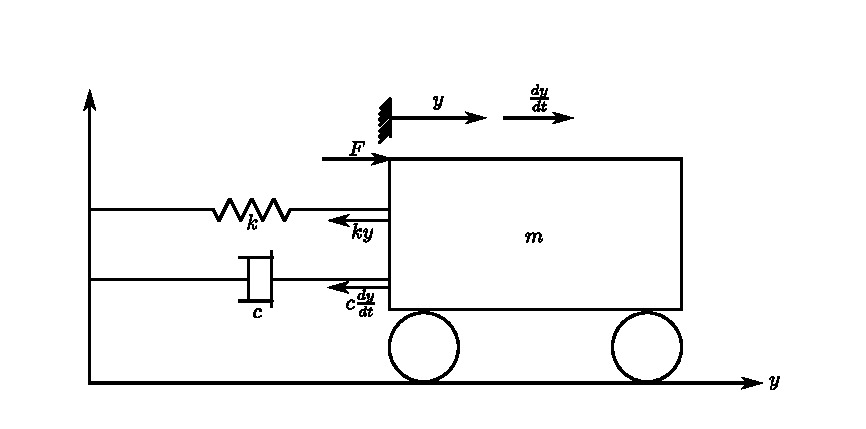
\includegraphics[scale=1]{src/img1.pdf}
	\end{figure}

	\begin{itemize}
		\item Step 1 : Obtain Equation of Motion. From the 2nd law of Newton:
	\end{itemize}
	\[
	\sum \vec{F} = m\vec{a}
	\]
	\[
	\begin{split}
		F - ky - c \dot{y} &= m \ddot{y} \\
		m \ddot{y} + c \dot{y} + ky &= F \\
		\ddot{y} + \frac{c}{m} \dot{y} + \frac{k}{m} y &= \frac{F}{m}
	\end{split}
	\]
	\begin{itemize}
		\item Step 2 : Choose State Variables. We would like to know \(y\) and \(\dot{y}\). Thus, Let Choose:
	\end{itemize}
	\[
	\begin{split}
		X_1 &= y \\
		X_2 &= \dot{y}
	\end{split}
	\]
	\begin{itemize}
		\item Step 3 : Take Derivative of State Vector.
	\end{itemize}
	\[
	\begin{split}
		X_1 &= y => \dot{X}_1 = \dot{y}\\
		X_2 &= \dot{y} => \dot{X}_2 = \ddot{y} = \frac{F}{m} - \frac{c}{m} \dot{y} - \frac{k}{m} y
	\end{split}
	\]
	\[
	\begin{bmatrix}
		\dot{X}_1 \\
		\dot{X}_2 
	\end{bmatrix} =
	\begin{bmatrix}
		\dot{y}                                           \\
		\frac{F}{m} - \frac{c}{m} \dot{y} - \frac{k}{m} y 
	\end{bmatrix}
	\]
	\begin{itemize}
		\item Step 4 : Write in State-Space form.
	\end{itemize}
	\[
	\dot{X} = 
	\begin{bmatrix}
		\dot{X}_1 \\
		\dot{X}_2 
	\end{bmatrix} =
	\begin{bmatrix}
		0            &   & 1            \\
		\frac{-k}{m} &   & \frac{-c}{m} 
	\end{bmatrix}
	\begin{bmatrix}
		X_1 \\
		X_2 
	\end{bmatrix} +
	\begin{bmatrix}
		0           \\
		\frac{1}{m} 
	\end{bmatrix} F
	\]
	\begin{itemize}
		\item Step 5 : Write Output Equation.
	\end{itemize}
	\[
	y =
	\begin{bmatrix}
		1 &   & 0 
	\end{bmatrix}
	\begin{bmatrix}
		X_1 \\
		X_2 
	\end{bmatrix}
	\]
	
	
	\subsection{Example 3}
	Ex : Obtain S.S from system of mass, spring with 2 vertical mass .
	\begin{figure}[]
		\centering
		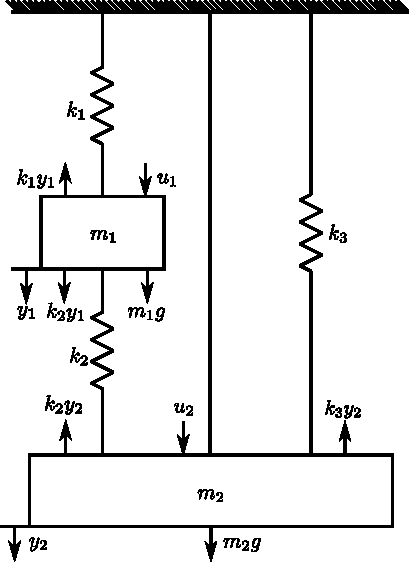
\includegraphics[scale=1]{src/img2.pdf}
	\end{figure}
	\begin{itemize}
		\item Step 1 : Obtain Equation of Motion. From the 2nd law of Newton:
	\end{itemize}
	\[
	\sum \vec{F} = m\vec{a}
	\]
	\[
	\begin{split}
		\text{Mass 1: } -k_1y_1 + k_2y_1 + u_1 + k_2y_2 = m_1\ddot{y}_1 \\
		\text{Mass 2: } -k_3y_2 - k_2y_2 + u_2 + k_2y_1 = m_2\ddot{y}_2
	\end{split}
	\]
	\begin{itemize}
		\item Step 2 : Choose State Variables. We would like to know \(y\) and \(\dot{y}\). Thus, Let Choose:
	\end{itemize}
	\[
	\begin{split}
		X_1 &= y_1 \\
		X_2 &= \dot{y}_1 \\
		X_3 &= y_2 \\
		X_4 &= \dot{y}_2
	\end{split}
	\]
	\begin{itemize}
		\item Step 3 : Take Derivative of State Vector.
	\end{itemize}
	\[
	\begin{split}
		X_1 &= y_1 => \dot{X}_1 = \dot{y}_1 \\
		X_2 &= \dot{y}_1 => \dot{X}_2 = \ddot{y}_1 = -\frac{k_1}{m_1}y_1 + \frac{k_2}{m_1}y_1 + \frac{1}{m_1}u_1 + \frac{k_2}{m_1}y_2 = \frac{k_2 - k_1}{m_1}y_1 + \frac{1}{m_1}u_1 + \frac{k_2}{m_1}y_2 \\
		X_3 &= y_2 => \dot{X}_3 = \dot{y}_2 \\ 
		X_4 &= \dot{y}_2 => \dot{X}_4 = \ddot{y}_2 = -\frac{k_3}{m_2}y_2 - \frac{k_2}{m_2}y_2 + \frac{1}{m_2}u_2 + \frac{k_2}{m_2}y_1 = \frac{-k_3 - k_2}{m_2}y_2 + \frac{1}{m_2}u_2 + \frac{k_2}{m_2}y_1
	\end{split}
	\]
	\[
	\begin{bmatrix}
		\dot{X}_1 \\
		\dot{X}_2 \\
		\dot{X}_3 \\
		\dot{X}_4 
	\end{bmatrix} =
	\begin{bmatrix}
		\dot{y}_1                                                         \\
		\frac{k_2 - k_1}{m_1}y_1 + \frac{1}{m_1}u_1 + \frac{k_2}{m_1}y_2  \\
		\dot{y}_2                                                         \\
		\frac{-k_3 - k_2}{m_2}y_2 + \frac{1}{m_2}u_2 + \frac{k_2}{m_2}y_1 
	\end{bmatrix}
	\]
	\begin{itemize}
		\item Step 4 : Write in State-Space form.
	\end{itemize}
	\[
	\dot{X} = 
	\begin{bmatrix}
		\dot{X}_1 \\
		\dot{X}_2 \\
		\dot{X}_3 \\
		\dot{X}_4 
	\end{bmatrix} =
	\begin{bmatrix}
		0                     &   & 1 &   & 0                      &   & 0 \\
		\frac{k_2 - k_1}{m_1} &   & 0 &   & \frac{k_2}{m_1}        &   & 0 \\
		0                     &   & 0 &   & 0                      &   & 1 \\
		\frac{k_2}{m_2}       &   & 0 &   & \frac{-k_3 - k_2}{m_2} &   & 0 \\
	\end{bmatrix}
	\begin{bmatrix}
		X_1 \\
		X_2 \\
		X_3 \\
		X_4 
	\end{bmatrix} +
	\begin{bmatrix}
		0             &   & 0             \\
		\frac{1}{m_1} &   & 0             \\
		0             &   & 0             \\
		0             &   & \frac{1}{m_2} 
	\end{bmatrix}
	\begin{bmatrix}
		u_1 \\
		u_2 
	\end{bmatrix}
	\]
	\begin{itemize}
		\item Step 5 : Write Output Equation.
	\end{itemize}
	\[
	y =
	\begin{bmatrix}
		1 &   & 0 &   & 0 &   & 0 \\ 
		0 &   & 0 &   & 1 &   & 0 \\ 
	\end{bmatrix}
	\begin{bmatrix}
		X_1 \\
		X_2 \\
		X_3 \\
		X_4 
	\end{bmatrix}
	\]
	
	\subsection{Example 4}
	Example : Solve system of single mass and spring and force using Matlab. MATLAB Numerical Method using ode45(Runge Kutta)
	\begin{lstlisting}[language=MATLAB]
		[t,x] = ode45(@f,tspan,x_0)
		t = time
		x = state vector
		ode45 = solver
		f = function
		tspan = t_0 -> t_f
		x_0 = initial condition
		
		
		Example:
		
		tspan = [0,10];
		x_0 = [0,0];
		
		function dx = model(t,x)
		% dx = Ax+Bu
		k = 0.01;m=1;u=2;
		A = [0 1;-k/m 0];
		B = [0;1/m];
		dx = A*x + B*u;
		
		[t,x] = ode45(@model,tspan,x_0);
		plot(t,x(:;1))
		hold on
		plot(t,x(:;2))
		legend('displacement','velocity')
	\end{lstlisting}
	
	\subsection{Example 5}
	Ex : Obtain S.S from system of mass, spring, damper with 2 horizontal mass .
	\begin{figure}[]
		\centering
		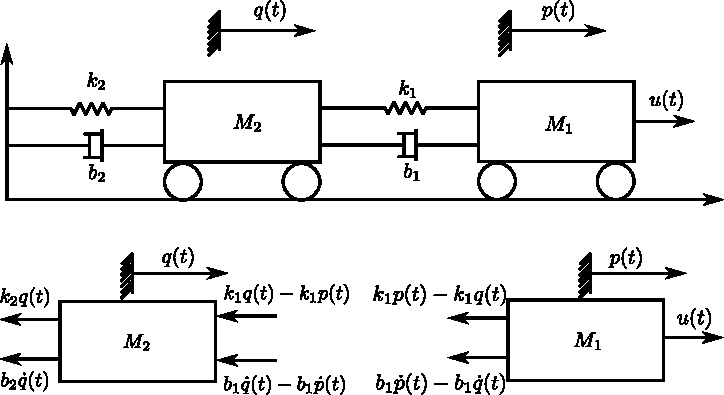
\includegraphics[scale=1]{src/img3.pdf}
	\end{figure}
	Equation of Motion
	\[
	\sum \vec{F} = m\vec{a}
	\]
	\[
	\begin{split}
		\text{Mass 1: }& m_1\ddot{p}(t) + b_1\dot{p}(t) + k_1p(t) = u(t) +k_1q(t)+b_1\dot{q}(t) \\
		\text{Mass 2: }& m_2\ddot{q}(t) + (k_1+k_2)q(t) + (b_1+b_2)\dot{q}(t) = k_1p(t)+b_1\dot{p}(t) \\
		&\ddot{p}(t)= \frac{1}{m_1}u(t) +\frac{k_1}{m_1}q(t)+\frac{b_1}{m_1}\dot{q}(t) - \frac{b_1}{m_1}\dot{p}(t) - \frac{k_1}{m_1}p(t)\\
		&\ddot{q}(t)= \frac{k_1}{m_2}p(t)+\frac{b_1}{m_2}\dot{p}(t) - \frac{(k_1+k_2)}{m_2}q(t) - \frac{(b_1+b_2)}{m_2}\dot{q}(t)
	\end{split}
	\]
	Let:
	\[
	x = 
	\begin{bmatrix}
		x_1 \\
		x_2 \\
		x_3 \\
		x_4 
	\end{bmatrix}
	= 
	\begin{bmatrix}
		p       \\
		q       \\
		\dot{p} \\
		\dot{q} 
	\end{bmatrix}
	=>
	\dot{x} = 
	\begin{bmatrix}
		\dot{x}_1 \\
		\dot{x}_2 \\
		\dot{x}_3 \\
		\dot{x}_4 
	\end{bmatrix}
	= 
	\begin{bmatrix}
		\dot{p}  \\
		\dot{q}  \\
		\ddot{p} \\
		\ddot{q} 
	\end{bmatrix}
	\]
	Thus, we get state space form:
	\[
	\dot{x} = 
	\begin{bmatrix}
		\dot{x}_1 \\
		\dot{x}_2 \\
		\dot{x}_3 \\
		\dot{x}_4 
	\end{bmatrix} =
	\begin{bmatrix}
		0                 &   & 0                       &   & 1                 &   & 0                       \\
		0                 &   & 0                       &   & 0                 &   & 1                       \\
		- \frac{k_1}{m_1} &   & \frac{k_1}{m_1}         &   & - \frac{b_1}{m_1} &   & \frac{b_1}{m_1}         \\
		\frac{k_1}{m_2}   &   & - \frac{(k_1+k_2)}{m_2} &   & \frac{b_1}{m_2}   &   & - \frac{(b_1+b_2)}{m_2} 
	\end{bmatrix}
	\begin{bmatrix}
		x_1 \\
		x_2 \\
		x_3 \\
		x_4 
	\end{bmatrix} +
	\begin{bmatrix}
		0             \\
		0             \\
		\frac{1}{m_1} \\
		0             
	\end{bmatrix} u(t)
	\]
	
	\[
	y =
	\begin{bmatrix}
		1 &   & 0 &   & 0 &   & 0 
	\end{bmatrix}
	\begin{bmatrix}
		x_1 \\
		x_2 \\
		x_3 \\
		x_4 
	\end{bmatrix}
	\]
	
	
	
	
	\section{State Space of Scalar Differential Equation System}
	
	\subsection{Case 1}
	Consider equation below:
	\[
	y^{(n)} + a_1y^{(n-1)} + ... + a_{n-1}y' + a_n y = u  \leftarrow \text{Input has not derivative}
	\]
	Let:
	\[
	x = 
	\begin{bmatrix}
		x_1     \\
		x_2     \\
		\vdots  \\
		x_{n-1} \\
		x_n     
	\end{bmatrix}
	=
	\begin{bmatrix}
		y       \\
		y'      \\
		\vdots  \\
		y^{n-1} \\
		y^n     
	\end{bmatrix}
	\]
	Thus
	\[
	\dot{x} = 
	\begin{bmatrix}
		\dot{x}_1     \\
		\dot{x}_2     \\
		\vdots        \\
		\dot{x}_{n-1} \\
		\dot{x}_n     
	\end{bmatrix}
	=
	\begin{bmatrix}
		y'                                \\
		y''                               \\
		\vdots                            \\
		y^n                               \\
		-a_0x_1 - a_1x_2 ... - a_nx_n + u 
	\end{bmatrix}
	=
	\begin{bmatrix}
		\dot{x}_2                         \\
		\dot{x}_3                         \\
		\vdots                            \\
		\dot{x}_n                         \\
		-a_0x_1 - a_1x_2 ... - a_nx_n + u 
	\end{bmatrix}
	\]
	Arrange into SS form:
	\[
	\dot{x} = 
	\begin{bmatrix}
		0      &   & 1        &   & 0        &   & ... &   & 0      \\
		0      &   & 0        &   & 1        &   & ... &   & 0      \\
		\vdots &   & \vdots   &   & \vdots   &   & ... &   & \vdots \\
		-a_n   &   & -a_{n-1} &   & -a_{n-2} &   & ... &   & -a_1   
	\end{bmatrix}
	\begin{bmatrix}
		x_1    \\
		x_2    \\
		\vdots \\
		x_n    
	\end{bmatrix} +
	\begin{bmatrix}
		0      \\
		0      \\
		\vdots \\
		1      
	\end{bmatrix} u
	\]
	\[
	y =
	\begin{bmatrix}
		1 &   & 0 &   & ... &   & 0 
	\end{bmatrix}
	\begin{bmatrix}
		x_1    \\
		x_2    \\
		\vdots \\
		x_n    
	\end{bmatrix}
	\]
	We have a corresponding Transfer Function is 
	\[\frac{Y(s)}{U(s)} = \frac{1}{s^n+a_1s^{n-1}+...+a_{n-1}s+a_n}\]
	
	\subsection{Case 2}
	Consider equation below:
	\[
	y^{(n)} + a_1y^{(n-1)} + ... + a_{n-1}y' + a_n y = \beta_0u^n + \beta_1u^{n-1}+ ... +\beta_nu  \leftarrow \text{Input has derivative}
	\]
	Let:
	\[
	\begin{split}
		x_1 &= y - \beta_0 u \\
		x_2 &= y' - \beta_0 u' - \beta_1 u = x'_1-\beta_1u \\
		\vdots \\
		x_n &= y^{n-1} - \beta_0 u^{n-1} - ... - \beta_{n-1} u = x'_{n-1}-\beta_{n-1}u
	\end{split}
	\]
	Where \(\beta_0 , \beta_1 , ... , \beta_{n-1}\) are determined from:
	\[
	\begin{split}
		\beta_0 &= b_0 \\
		\beta_1 &= b_1 - a_1\beta_0 \\
		\beta_2 &= b_2 - a_1\beta_1 - a_2\beta_0 \\
		\vdots
	\end{split}
	\]
	Arrange into SS form:
	\[
	\dot{x} = 
	\begin{bmatrix}
		0      &   & 1        &   & 0        &   & ... &   & 0      \\
		0      &   & 0        &   & 1        &   & ... &   & 0      \\
		\vdots &   & \vdots   &   & \vdots   &   & ... &   & \vdots \\
		-a_n   &   & -a_{n-1} &   & -a_{n-2} &   & ... &   & -a_1   
	\end{bmatrix}
	\begin{bmatrix}
		x_1    \\
		x_2    \\
		\vdots \\
		x_n    
	\end{bmatrix} +
	\begin{bmatrix}
		\beta_1 \\
		\beta_2 \\
		\vdots  \\
		\beta_n 
	\end{bmatrix} u
	\]
	\[
	y =
	\begin{bmatrix}
		1 &   & 0 &   & ... &   & 0 
	\end{bmatrix}
	\begin{bmatrix}
		x_1    \\
		x_2    \\
		\vdots \\
		x_n    
	\end{bmatrix} + \beta_0 u
	\]
	We have a corresponding Transfer Function is 
	\[\frac{Y(s)}{U(s)} = \frac{b_0 s^n + b_1s^{n-1} + ... + b_{n-1}s+ b_n}{s^n+a_1s^{n-1}+...+a_{n-1}s+a_n}\]
	
	
	\section{Transfer Function to State Space}
	Example:
	\[\frac{Y(s)}{U(s)} = \frac{100}{s^4 + 20s^3 + 10s^2 + 7s + 100}\]
	\[(s^4 + 20s^3 + 10s^2 + 7s + 100)Y(s) = 100 U(s)\]
	Taking Inverse Laplace Transform
	\[y^{(4)} + 20y^{(3)} + 10 y'' + 7y' + 100y = 100 u\]
	Let:
	\[
	\begin{split}
		x_1 &= y   => \dot{x}_1 = y' = x_2\\
		x_2 &= y'  => \dot{x}_2 = y'' = x_3\\
		x_3 &= y'' => \dot{x}_3 = y^{(3)} = x_4\\
		x_3 &= y'''=> \dot{x}_4 = y^{(4)} = 100u - 20y^{(3)} - 10 y'' - 7y' - 100y
	\end{split}
	\]
	State Space form:
	\[
	\dot{x} = 
	\begin{bmatrix}
		0    &   & 1  &   & 0   &   & 0   \\
		0    &   & 0  &   & 1   &   & 0   \\
		0    &   & 0  &   & 0   &   & 1   \\
		-100 &   & -7 &   & -10 &   & -20 
	\end{bmatrix}
	\begin{bmatrix}
		x_1 \\
		x_2 \\
		x_3 \\
		x_4 
	\end{bmatrix} + 
	\begin{bmatrix}
		0   \\
		0   \\
		0   \\
		100 
	\end{bmatrix} u
	\]
	\[
	y =
	\begin{bmatrix}
		1 &   & 0 &   & 0 &   & 0 
	\end{bmatrix}
	\begin{bmatrix}
		x_1 \\
		x_2 \\
		x_3 \\
		x_4 
	\end{bmatrix}
	\]
	
	
	\section{State Space to Transfer Function}
	We have a Transfer Function:
	\[
	\frac{Y(s)}{U(s)} = G(s)
	\]
	with state space in form of:
	\[
	\begin{split}
		\dot{x} &= Ax + Bu \\
		y &= Cx + Du
	\end{split}
	\]
	Let have a Laplace transform of SS:
	\[
	\begin{split}
		sX(s)-x(0) &= AX(s) + BU(s) \\
		Y(s) &= CX(s) + DU(s)
	\end{split}
	\]
	Assuming \(x(0) = 0 IC\), we get:
	\[
	\begin{split}
		sX(s) - AX(s) &= BU(s) \\
		(sI - A)X(s) &= BU(s) \\
		(sI - A)^{-1}(sI - A)X(s) &= (sI - A)^{-1}BU(s) \\
		X(s) &= (sI - A)^{-1}BU(s)
	\end{split}
	\]
	Substitute into \(Y(s)\)
	\[
	\begin{split}
		Y(s) &= C[(sI - A)^{-1}BU(s)] + DU(s) \\
		Y(s) &= C(sI - A)^{-1}BU(s) + DU(s) \\
		Y(s) &= [C(sI - A)^{-1}B + D]U(s)
	\end{split}
	\]
	Thus the Transfer function can be found by:
	\[
	G(s) = C(sI - A)^{-1}B + D
	\]
	Example:
	\[
	\dot{x} = 
	\begin{bmatrix}
		0  &   & 1   &   & 0  \\
		0  &   & 0   &   & 1  \\
		-5 &   & -25 &   & -5 
	\end{bmatrix}
	\begin{bmatrix}
		x_1 \\
		x_2 \\
		x_3 
	\end{bmatrix} + 
	\begin{bmatrix}
		0    \\
		25   \\
		-120 
	\end{bmatrix} u
	\]
	\[
	y =
	\begin{bmatrix}
		1 &   & 0 &   & 0 
	\end{bmatrix}
	\begin{bmatrix}
		x_1 \\
		x_2 \\
		x_3 
	\end{bmatrix}
	\]
	
	\[
	G(s) = 
	\begin{bmatrix}
		1 &   & 0 &   & 0 
	\end{bmatrix}
	[
	\begin{bmatrix}
		s &   & 0 &   & 0 \\
		0 &   & s &   & 0 \\
		0 &   & 0 &   & s 
	\end{bmatrix}
	-
	\begin{bmatrix}
		0  &   & 1   &   & 0  \\
		0  &   & 0   &   & 1  \\
		-5 &   & -25 &   & -5 
	\end{bmatrix}]^{-1}
	\begin{bmatrix}
		0    \\
		25   \\
		-120 
	\end{bmatrix} + 0
	\]
	
	\[
	G(s) = 
	\begin{bmatrix}
		1 &   & 0 &   & 0 
	\end{bmatrix}
	\begin{bmatrix}
		s  &   & 1   &   & 0   \\
		0  &   & s   &   & 1   \\
		-5 &   & -25 &   & s+5 
	\end{bmatrix}^{-1}
	\begin{bmatrix}
		0    \\
		25   \\
		-120 
	\end{bmatrix}
	\]
	
	\[
	G(s) = 
	\begin{bmatrix}
		1 &   & 0 &   & 0 
	\end{bmatrix}
	\begin{bmatrix}
		\frac{(s^2+5s+25)}{(s^3+5s^2+25s-5)} &   & \frac{(-s-5)}{(s^3+5s^2+25s-5)}   &   & \frac{1}{(s^3+5s^2+25s-5)}   \\
		\frac{-5}{(s^3+5s^2+25s-5)}          &   & \frac{(s^2+5s)}{(s^3+5s^2+25s-5)} &   & \frac{-s}{(s^3+5s^2+25s-5)}  \\
		\frac{5s}{(s^3+5s^2+25s-5)}          &   & \frac{(25s-5)}{(s^3+5s^2+25s-5)}  &   & \frac{s^2}{(s^3+5s^2+25s-5)} 
	\end{bmatrix}
	\begin{bmatrix}
		0    \\
		25   \\
		-120 
	\end{bmatrix}
	\]
	
	\[
	G(s) = 
	\begin{bmatrix}
		1 &   & 0 &   & 0 
	\end{bmatrix}
	\begin{bmatrix}
		\frac{(-25s-245)}{(s^3+5s^2+25s-5)}         \\
		\frac{(25s^2+245s)}{(s^3+5s^2+25s-5)}       \\
		\frac{(-120s^2+625s-125)}{(s^3+5s^2+25s-5)} 
	\end{bmatrix}
	\]
	
	\[
	G(s) = \frac{(-25s-245)}{(s^3+5s^2+25s-5)}
	\]
	
	
	Thus
	\[
	G(s) = \frac{25s + 245}{s^3 + 5s^2 + 25s + 5}
	\]
	
	
\end{document}